\chapter{What Things Are Made Of}\label{ch:g1:materials-around-us}

Look at a breakfast table. There is a spoon, a glass of milk, a fork, a
napkin, a bowl, and a jumper hanging on the back of a chair. That is
many things, and each one is made of something: the spoon of wood, the
fork of metal, the glass of glass, the napkin of paper, the bowl of
plastic, the jumper of wool. A table full of things, made of only a
handful of different stuffs. This chapter is about those stuffs.

\begin{omfigure}
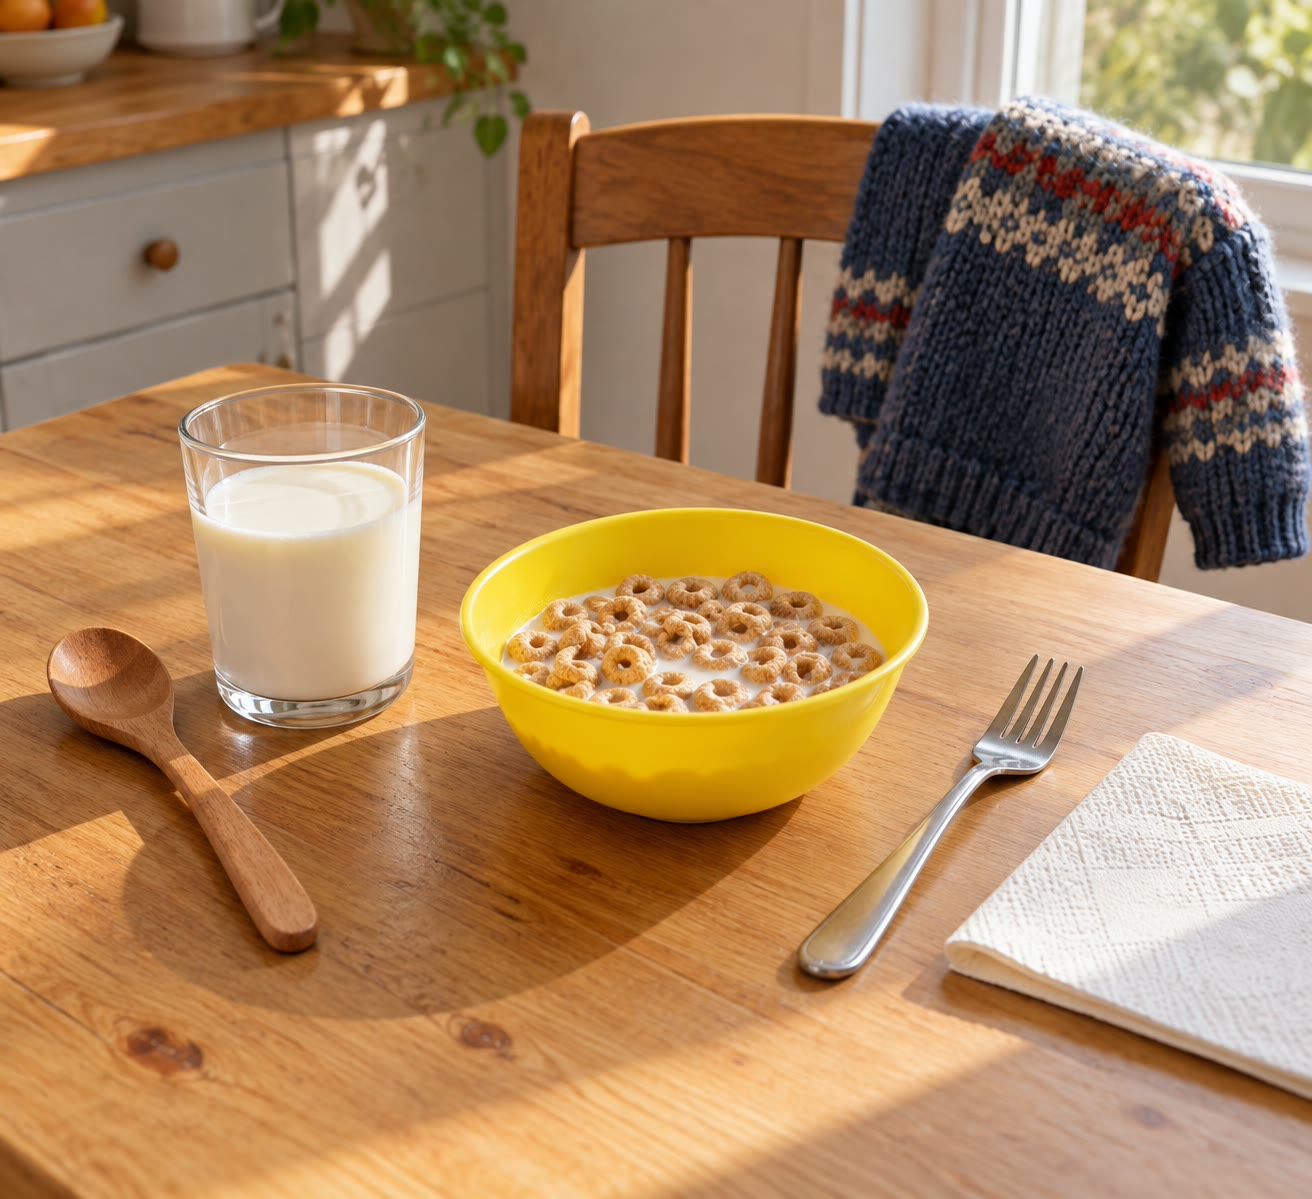
\includegraphics[width=0.62\linewidth]{images/book1/ai/g1-breakfast-table.jpg}

{\small A breakfast table: many \omterm{def:g1:materials-around-us:object}{objects}, made of a few \omterm{def:g1:materials-around-us:material}{materials}.}
\end{omfigure}

\section{Objects and materials}

\begin{definition}[Object]\label{def:g1:materials-around-us:object}
An \emph{object}\index{object} is a thing we can see and touch, and
often hold and use: a spoon, a chair, a ball, a window, a shoe.
\end{definition}

\begin{definition}[Material]\label{def:g1:materials-around-us:material}
The \emph{material}\index{material} of an \omterm{def:g1:materials-around-us:object}{object} is what the \omterm{def:g1:materials-around-us:object}{object} is
made of. A spoon can be made of wood, of metal or of plastic: the spoon
is the \omterm{def:g1:materials-around-us:object}{object}, the wood is the material.
\end{definition}

\begin{example}[One object, three materials]\label{ex:g1:materials-around-us:spoons}
Three spoons lie side by side. They have the same shape and do the same
job, so they are the same kind of \omterm{def:g1:materials-around-us:object}{object}. But one is made of wood, one
of metal and one of plastic: three different \omterm{def:g1:materials-around-us:material}{materials}.
\end{example}

\begin{omfigure}
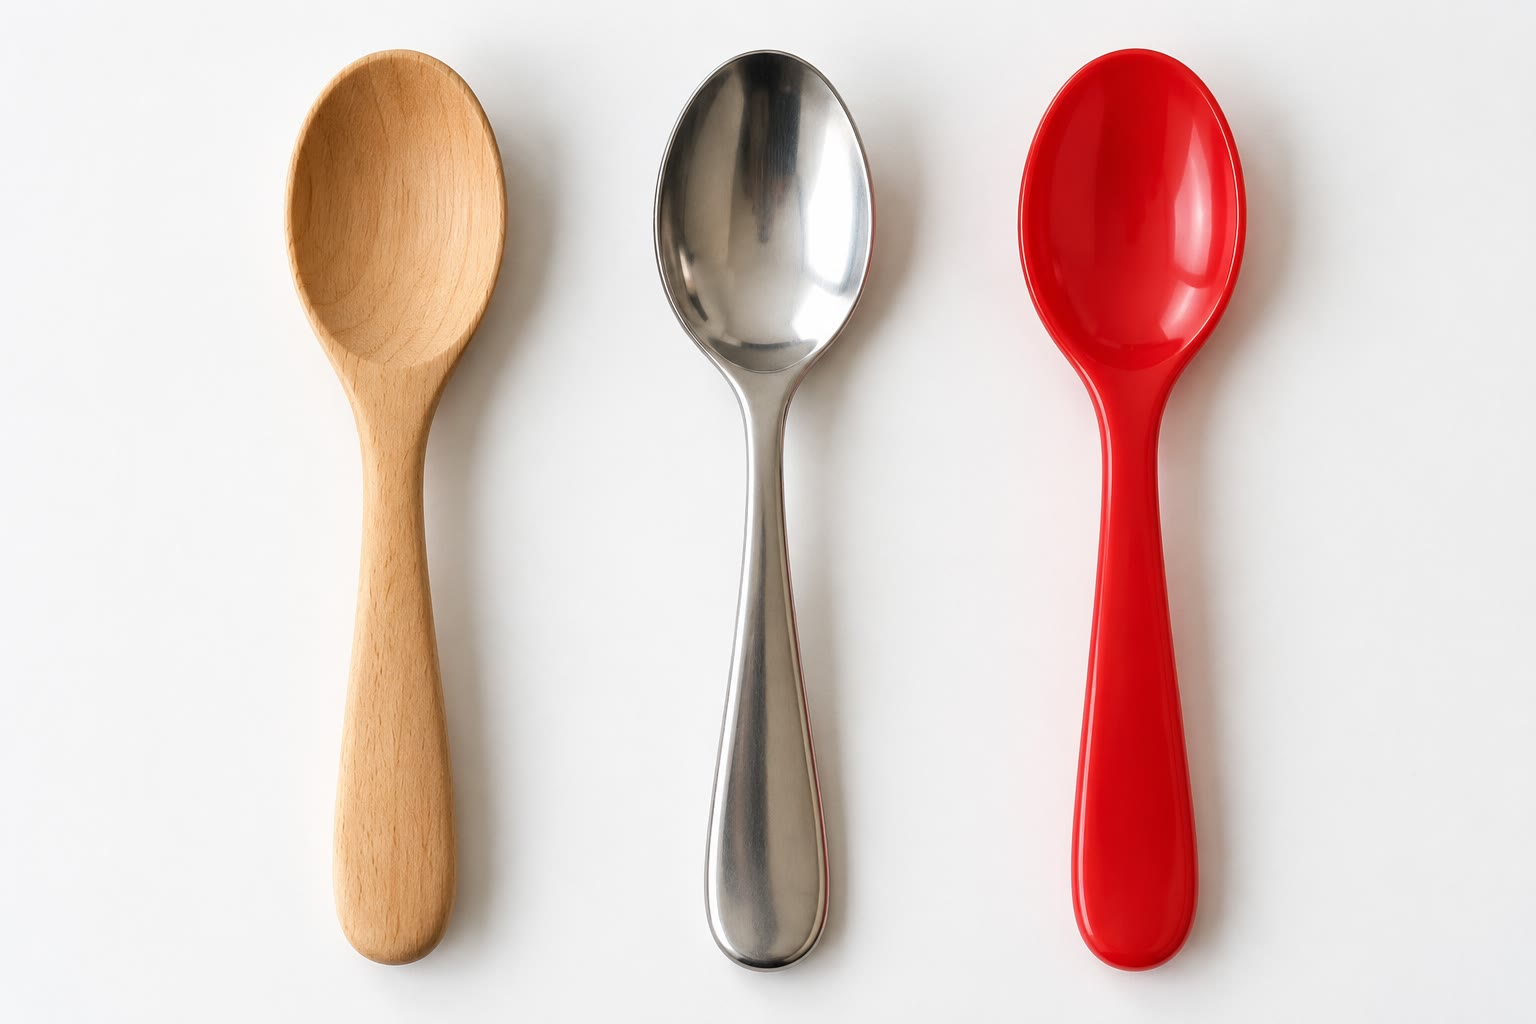
\includegraphics[width=0.55\linewidth]{images/book1/ai/g1-three-spoons.jpg}

{\small Three spoons: the same \omterm{def:g1:materials-around-us:object}{object}, three \omterm{def:g1:materials-around-us:material}{materials} --- wood, metal
and plastic.}
\end{omfigure}

\begin{example}[One material, many objects]\label{ex:g1:materials-around-us:wood}
Wood is the \omterm{def:g1:materials-around-us:material}{material} of a pencil, a chair, a door, a toy train and a
wooden spoon. Many different \omterm{def:g1:materials-around-us:object}{objects} can be made of the same \omterm{def:g1:materials-around-us:material}{material}.
\end{example}

\begin{remark}[Objects made of several materials]\label{rem:g1:materials-around-us:several}
Many \omterm{def:g1:materials-around-us:object}{objects} are made of more than one \omterm{def:g1:materials-around-us:material}{material}. A pair of scissors
has blades of metal and handles of plastic. A pencil is wood outside
and a grey stick of graphite inside. A window is glass in a frame of
wood, metal or plastic.
\end{remark}

\section{Seven common materials}

\begin{proposition}[Materials all around us]\label{prop:g1:materials-around-us:seven}
Most of the \omterm{def:g1:materials-around-us:object}{objects} around us are made of a few common \omterm{def:g1:materials-around-us:material}{materials}:
\begin{itemize}
  \item \textbf{wood}: tables, chairs, pencils, doors;
  \item \textbf{metal}: forks, keys, nails, pans, bicycles;
  \item \textbf{glass}: windows, jars, bottles, glasses;
  \item \textbf{plastic}: bowls, bottles, toys, buckets;
  \item \textbf{paper} and card: books, napkins, boxes;
  \item \textbf{fabric}: clothes, curtains, bags --- made of wool,
        cotton or other threads;
  \item \textbf{stone}: walls, steps, pebbles, statues.
\end{itemize}
\end{proposition}

\begin{omfigure}
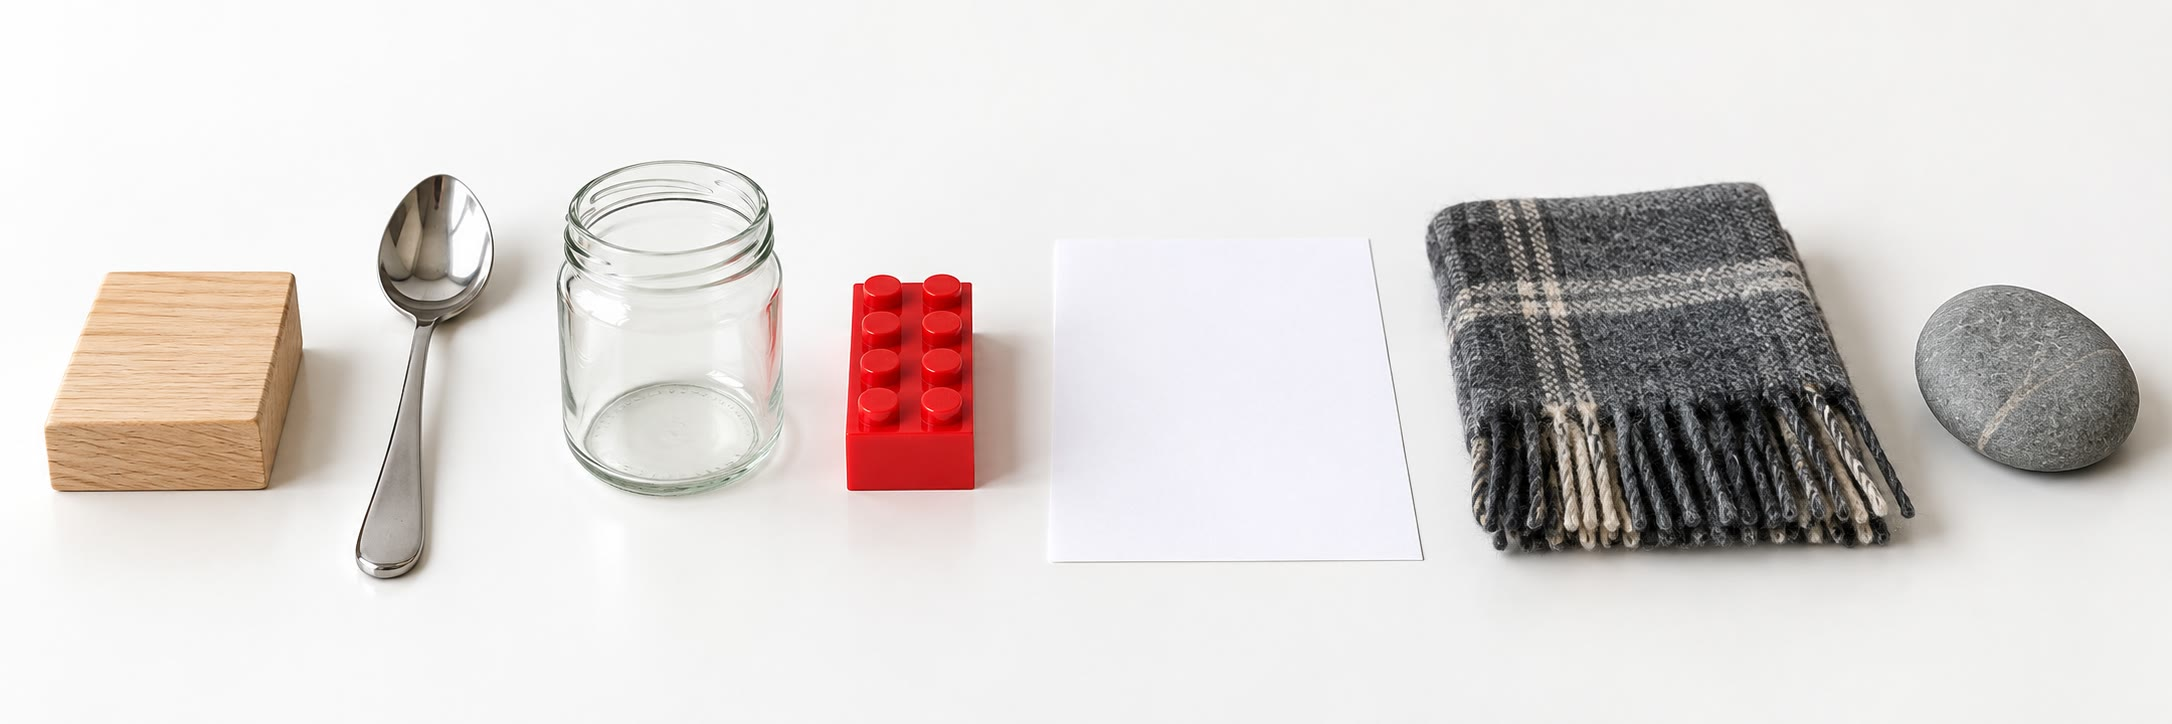
\includegraphics[width=0.75\linewidth]{images/book1/ai/g1-material-samples.jpg}

{\small Seven samples, from left to right: wood, metal, glass, plastic,
paper, fabric (wool) and stone.}
\end{omfigure}

\begin{remark}[Names that are also materials]\label{rem:g1:materials-around-us:names}
We call a drinking glass ``a glass'' because it is made of glass, and a
sheet of paper ``a paper''. The word for the \omterm{def:g1:materials-around-us:object}{object} and the word for the
\omterm{def:g1:materials-around-us:material}{material} are then the same. When we speak of \omterm{def:g1:materials-around-us:material}{materials}, we mean the
stuff, not the \omterm{def:g1:materials-around-us:object}{object}.
\end{remark}

\section{Properties of materials}

\begin{definition}[Property of a material]\label{def:g1:materials-around-us:property}
A \emph{property of a material}\index{property of a material} is
something we can find out about it by looking, touching or testing: is
it hard or soft? Can we see through it? Does a magnet pull it? Does it
float on water or sink?
\end{definition}

\begin{example}[Hard and soft]\label{ex:g1:materials-around-us:hard}
A pebble is hard: pressing it with a thumb leaves no mark. A wool scarf
is soft: it bends and folds in the hand. Wood, metal, glass and stone
are hard; fabric and paper are soft and bend easily.
\end{example}

\begin{example}[Seeing through]\label{ex:g1:materials-around-us:see-through}
We can see the garden through a window: glass lets light through, we
say it is \emph{transparent}. We cannot see through a wooden door, a
brick wall or a metal pan. Some plastics are transparent, like a water
bottle; others are not, like a red toy brick.
\end{example}

\begin{example}[Attracted by a magnet]\label{ex:g1:materials-around-us:magnet}
A magnet pulls a steel paper clip, a steel nail or an iron key towards
it. It does not pull wood, glass, plastic, paper, fabric or stone. And,
surprisingly, it does not pull every metal: a drink can of aluminium and
a copper wire stay where they are. A magnet attracts \omterm{def:g1:materials-around-us:object}{objects} made of iron
and of steel, which is mostly iron.
\end{example}

\begin{omfigure}
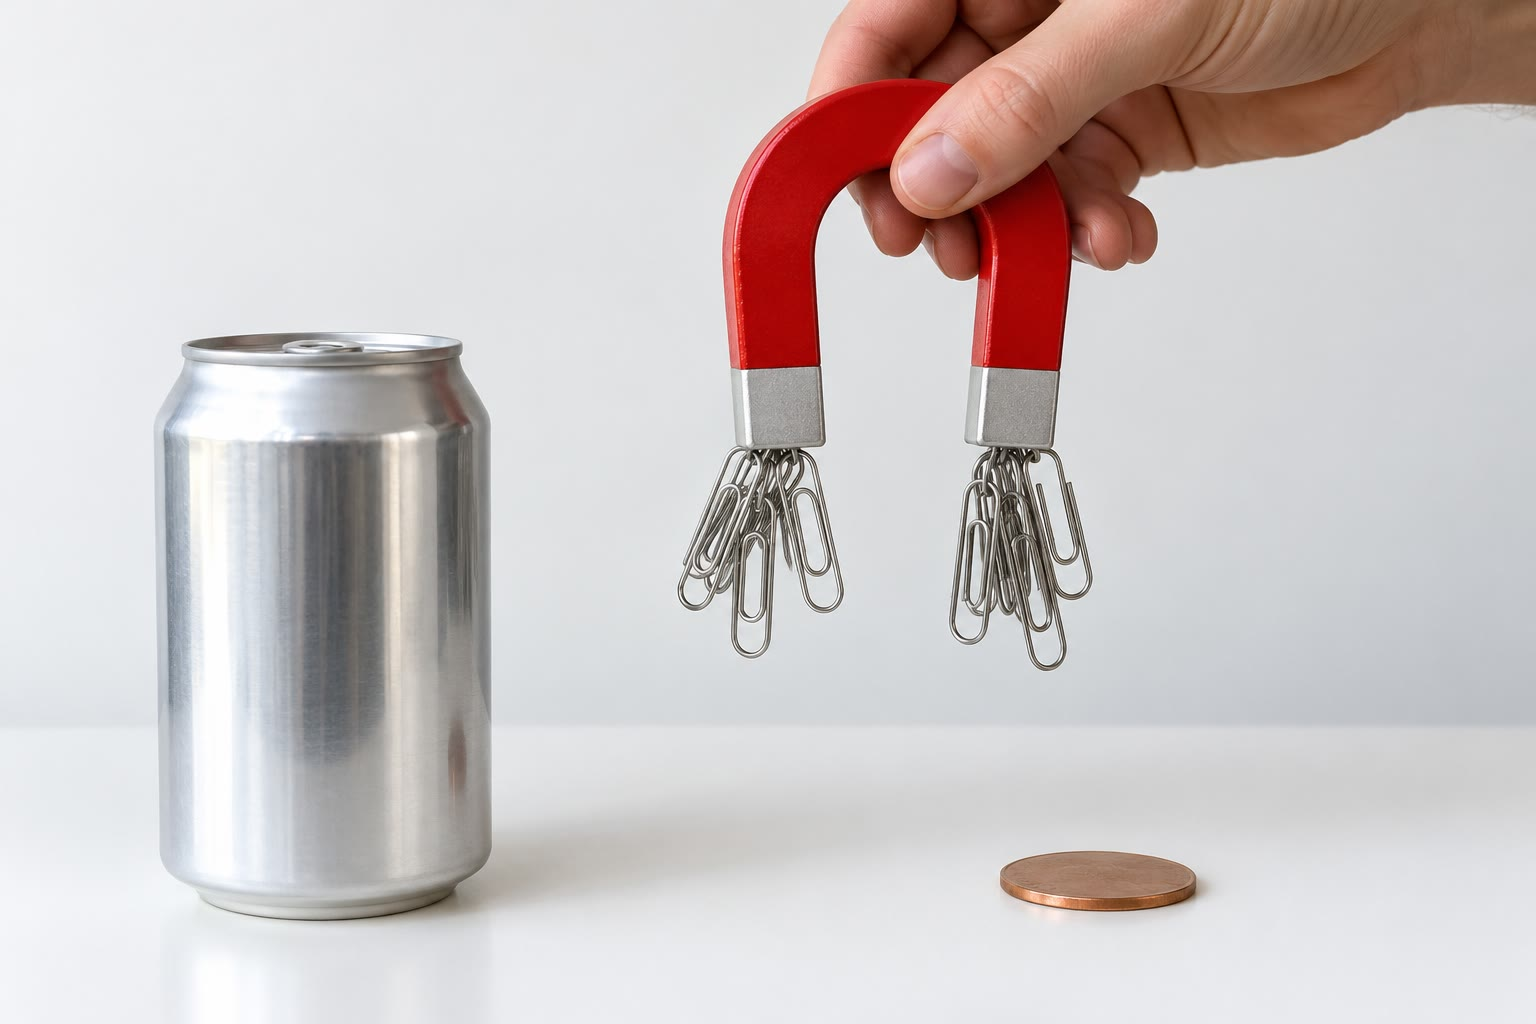
\includegraphics[width=0.55\linewidth]{images/book1/ai/g1-magnet-clips.jpg}

{\small A magnet lifts steel paper clips. The aluminium can and the
copper disc on the table stay where they are.}
\end{omfigure}

\begin{example}[Floating and sinking]\label{ex:g1:materials-around-us:float}
Put a few \omterm{def:g1:materials-around-us:object}{objects} in a basin of water. A wooden block and a plastic
bottle cap float. A pebble, a glass marble and a steel nail sink to the
bottom. Whether a thing floats or sinks is also a property of its
\omterm{def:g1:materials-around-us:material}{material}.
\end{example}

\begin{omfigure}
\begin{tikzpicture}[font=\small]
  % the basin
  \fill[omWater!80] (0,0) rectangle (9,2.2);
  \draw[omGlass, line width=0.8pt] (-0.1,2.7) -- (0,2.6) -- (0,0) -- (9,0)
    -- (9,2.6) -- (9.1,2.7);
  % floating: wooden block, plastic cap
  \fill[brown!55, draw=brown!70!black] (0.8,2.0) rectangle (2.2,2.5);
  \fill[red!70, draw=red!50!black] (3.7,2.05) rectangle (4.3,2.35);
  % sunk: pebble, marble, nail
  \fill[black!35, draw=black!60] (5.0,0.25) ellipse (0.45 and 0.22);
  \shade[ball color=cyan!40] (6.5,0.2) circle (0.18);
  \fill[black!55] (7.6,0.06) rectangle (8.6,0.14);
  \fill[black!55] (7.52,0.02) rectangle (7.62,0.18);
  % labels
  \node[anchor=south] at (1.5,2.75) {wooden block};
  \node[anchor=south] at (4.0,2.75) {plastic cap};
  \node[anchor=north] at (5.0,-0.1) {pebble};
  \node[anchor=north] at (6.5,-0.1) {marble};
  \node[anchor=north] at (8.1,-0.1) {nail};
  \node[anchor=west, align=left] at (9.3,2.2) {these float};
  \node[anchor=west, align=left] at (9.3,0.2) {these sink};
\end{tikzpicture}

{\small In a basin of water: the wooden block and the plastic cap float;
the pebble, the glass marble and the steel nail sink.}
\end{omfigure}

\section{Sorting materials}

\begin{method}[Sorting by one property]\label{met:g1:materials-around-us:sort}
To sort a pile of \omterm{def:g1:materials-around-us:object}{objects}:
\begin{enumerate}
  \item choose \textbf{one} question, for instance ``Does a magnet pull
        it?'';
  \item test each \omterm{def:g1:materials-around-us:object}{object} and put it in the ``yes'' group or the ``no''
        group;
  \item then, if you wish, sort each group again with another question.
\end{enumerate}
One question at a time: that way every \omterm{def:g1:materials-around-us:object}{object} has exactly one place.
\end{method}

\begin{omfigure}
\begin{tikzpicture}[font=\small]
  \draw[omDef, line width=1pt] (0,0) circle (2.3);
  \draw[omProp, line width=1pt] (2.4,0) circle (2.3);
  \node[omDef, font=\small\bfseries] at (-0.6,2.65) {made of metal};
  \node[omProp, font=\small\bfseries] at (3.0,2.65) {pulled by a magnet};
  \node[font=\footnotesize] at (-1.1,0.35) {drink can};
  \node[font=\footnotesize] at (-1.1,-0.35) {copper wire};
  \node[font=\footnotesize] at (1.2,0.6) {steel nail};
  \node[font=\footnotesize] at (1.2,0) {iron key};
  \node[font=\footnotesize] at (1.2,-0.6) {paper clip};
  \node[font=\footnotesize] at (3.5,0) {(nothing)};
  \node[anchor=west] at (5.2,0.9) {wooden spoon};
  \node[anchor=west] at (5.2,0.3) {glass marble};
  \node[anchor=west] at (5.2,-0.3) {wool scarf};
  \node[anchor=west] at (5.2,-0.9) {pebble};
\end{tikzpicture}

{\small Two questions, two hoops. Inside the blue hoop: the \omterm{def:g1:materials-around-us:object}{objects} made
of metal. Inside the orange hoop: the \omterm{def:g1:materials-around-us:object}{objects} a magnet pulls. In both
hoops: the \omterm{def:g1:materials-around-us:object}{objects} of iron or steel. Outside both: everything else.}
\end{omfigure}

\begin{center}
\small
\begin{tabular}{lccc}
\hline
\omterm{def:g1:materials-around-us:object}{object} (\omterm{def:g1:materials-around-us:material}{material}) & hard? & see-through? & pulled by a magnet? \\
\hline
block (wood) & yes & no & no \\
nail (steel) & yes & no & yes \\
marble (glass) & yes & yes & no \\
bottle cap (plastic) & yes & no & no \\
sheet (paper) & no & no & no \\
scarf (wool) & no & no & no \\
pebble (stone) & yes & no & no \\
\hline
\end{tabular}
\end{center}

\section{The right material for the job}

\begin{proposition}[Each material is chosen for its properties]\label{prop:g1:materials-around-us:choose}
People choose the \omterm{def:g1:materials-around-us:material}{material} of an \omterm{def:g1:materials-around-us:object}{object} for what the \omterm{def:g1:materials-around-us:object}{object} must do:
\begin{itemize}
  \item a window must let light in: it is made of glass, which is
        transparent;
  \item a raincoat must keep the rain out and fold up: it is made of
        plastic or of a fabric that water cannot pass through;
  \item a pan must not melt on the cooker: it is made of metal;
  \item a pan's handle must not burn the hand: it is often made of wood
        or of a hard plastic, which do not get as hot as metal;
  \item a pillow must be soft: it is made of fabric filled with feathers
        or fibres.
\end{itemize}
\end{proposition}

\begin{example}[A boat]\label{ex:g1:materials-around-us:boat}
A toy boat must float. It can be made of wood or of plastic. A boat made
of a solid lump of stone would sink at once.
\end{example}

\begin{remark}[Broken glass]\label{rem:g1:materials-around-us:glass}
Glass is hard but it breaks, and its pieces are sharp. When a glass
breaks, an adult picks up the pieces.
\end{remark}

\section{Exercises}

\begin{exercise}[$\star$]\label{exo:g1:materials-around-us:1}
Is a chair an \omterm{def:g1:materials-around-us:object}{object} or a \omterm{def:g1:materials-around-us:material}{material}? Is wood an \omterm{def:g1:materials-around-us:object}{object} or a \omterm{def:g1:materials-around-us:material}{material}?
\end{exercise}

\begin{exercise}[$\star$]\label{exo:g1:materials-around-us:2}
Name the \omterm{def:g1:materials-around-us:material}{material} of each \omterm{def:g1:materials-around-us:object}{object}: a window pane, a nail, a pebble, a
book, a sock.
\end{exercise}

\begin{exercise}[$\star$]\label{exo:g1:materials-around-us:3}
Give two \omterm{def:g1:materials-around-us:object}{objects} made of wood and two \omterm{def:g1:materials-around-us:object}{objects} made of plastic.
\end{exercise}

\begin{exercise}[$\star$]\label{exo:g1:materials-around-us:4}
Find the odd one out, and say why: a wooden spoon, a metal fork, a
plastic spoon, a wooden chair. (Look at the \omterm{def:g1:materials-around-us:material}{materials}.)
\end{exercise}

\begin{exercise}[$\star$]\label{exo:g1:materials-around-us:5}
Which \omterm{def:g1:materials-around-us:material}{material} can we see through: wood, glass or stone?
\end{exercise}

\begin{exercise}[$\star$]\label{exo:g1:materials-around-us:6}
A magnet is held near a steel nail, a glass marble and a wooden block.
Which one does it pull?
\end{exercise}

\begin{exercise}[$\star$]\label{exo:g1:materials-around-us:7}
Look at the figure with the basin. How many \omterm{def:g1:materials-around-us:object}{objects} float? How many
sink?
\end{exercise}

\begin{exercise}[$\star$]\label{exo:g1:materials-around-us:8}
A pair of scissors has blades and handles. Which \omterm{def:g1:materials-around-us:material}{material} is each part
made of? Is a pair of scissors made of one \omterm{def:g1:materials-around-us:material}{material} or of two?
\end{exercise}

\begin{exercise}[$\star$]\label{exo:g1:materials-around-us:9}
Look at the figure with the two hoops. In which hoop is the drink can?
Why is it not in the orange hoop?
\end{exercise}

\begin{exercise}[$\star\star$]\label{exo:g1:materials-around-us:10}
Why are windows made of glass and not of wood?
\end{exercise}

\begin{exercise}[$\star\star$]\label{exo:g1:materials-around-us:11}
Sam wants to sort these 8 \omterm{def:g1:materials-around-us:object}{objects} with the question ``Does a magnet pull
it?'': a steel nail, a paper clip, a pebble, a wooden spoon, an iron
key, a drink can, a glass marble, a wool sock. How many \omterm{def:g1:materials-around-us:object}{objects} go in the
``yes'' group? How many in the ``no'' group?
\end{exercise}
